I used the training data obtained from both of the vectorizers(\verb|CountVectorizer()| \& \verb|TfidfVectorizer()|) to train a variety of models using training data and then used testing data to measure various matrices regarding that particular model, most importantly the \textbf{accuracy}.
In order to obtain different metrics regarding a particular model, I used the \verb|classification_report()| method imported from \verb|sklearn.metrics|.

\subsection{Results}\label{subsec:results}
Below, I am attaching all the metrics found by different learning models.

Logistic Regression using \verb|CountVectorizer|
\begin{table}[H]
    \begin{tabular}{lllll}
        & precision & recall & f1-score                     & support \\
        NON-SPAM          & 0.99      & 0.99   & 0.99                         & 843     \\
        SPAM              & 0.98      & 0.97   & 0.98                         & 296     \\
        &           &        &                              &         \\
        \textbf{accuracy} &           &        & \cellcolor[HTML]{FFCCC9}0.99 & 1139
    \end{tabular}\label{tab:Logistic_count_vect}
\end{table}

Logistic Regression using \verb|TfidfVectorizer|
\begin{table}[H]
    \begin{tabular}{lllll}
        & precision & recall & f1-score                     & support \\
        NON-SPAM          & 0.97      & 0.99   & 0.98                         & 843     \\
        SPAM              & 0.96      & 0.91   & 0.93                         & 296     \\
        &           &        &                              &         \\
        \textbf{accuracy} &           &        & \cellcolor[HTML]{FFCCC9}0.96 & 1139
    \end{tabular}\label{tab:Logistic_tfidf_vect}
\end{table}

MultinomialNB using \verb|CountVectorizer|
\begin{table}[H]
    \begin{tabular}{lllll}
        & precision & recall & f1-score                     & support \\
        NON-SPAM          & 1.00      & 0.99   & 0.99                         & 843     \\
        SPAM              & 0.97      & 0.99   & 0.98                         & 296     \\
        &           &        &                              &         \\
        \textbf{accuracy} &           &        & \cellcolor[HTML]{FFCCC9}0.99 & 1139
    \end{tabular}\label{tab:Multinomial_count_vect}
\end{table}

MultinomialNB using \verb|TfidfVectorizer|
\begin{table}[H]
    \begin{tabular}{lllll}
        & precision & recall & f1-score                     & support \\
        NON-SPAM          & 0.83      & 1.00   & 0.91                         & 843     \\
        SPAM              & 1.00      & 0.43   & 0.60                         & 296     \\
        &           &        &                              &         \\
        \textbf{accuracy} &           &        & \cellcolor[HTML]{FFCCC9}0.85 & 1139
    \end{tabular}\label{tab:Multinomial_tfidf_vect}
\end{table}
For some reason there is a lot of difference in terms of accuracy between \verb|Count & Tfidf| Vectorizer when
using Multinomial Naive Bayes Model.


BernoulliNB using \verb|CountVectorizer|
\begin{table}[H]
    \begin{tabular}{lllll}
        & precision & recall & f1-score                     & support \\
        NON-SPAM          & 0.98      & 0.99   & 0.99                         & 843     \\
        SPAM              & 0.97      & 0.95   & 0.96                         & 296     \\
        &           &        &                              &         \\
        \textbf{accuracy} &           &        & \cellcolor[HTML]{FFCCC9}0.98 & 1139
    \end{tabular}\label{tab:BernoulliNB_count_vect}
\end{table}

BernoulliNB using \verb|TfidfVectorizer|
\begin{table}[H]
    \begin{tabular}{lllll}
        & precision & recall & f1-score                     & support \\
        NON-SPAM          & 0.98      & 0.99   & 0.99                         & 843     \\
        SPAM              & 0.97      & 0.95   & 0.96                         & 296     \\
        &           &        &                              &         \\
        \textbf{accuracy} &           &        & \cellcolor[HTML]{FFCCC9}0.98 & 1139
    \end{tabular}\label{tab:BernoulliNB_tfidf_vect}
\end{table}

GaussianNB using \verb|CountVectorizer|
\begin{table}[H]
    \begin{tabular}{lllll}
        & precision & recall & f1-score                     & support \\
        NON-SPAM          & 0.96      & 0.99   & 0.97                         & 843     \\
        SPAM              & 0.97      & 0.87   & 0.91                         & 296     \\
        &           &        &                              &         \\
        \textbf{accuracy} &           &        & \cellcolor[HTML]{FFCCC9}0.96 & 1139
    \end{tabular}\label{tab:GaussianNB_count_vect}
\end{table}

GaussianNB using \verb|TfidfVectorizer|
\begin{table}[H]
    \begin{tabular}{lllll}
        & precision & recall & f1-score                     & support \\
        NON-SPAM          & 0.95      & 0.99   & 0.97                         & 843     \\
        SPAM              & 0.98      & 0.86   & 0.92                         & 296     \\
        &           &        &                              &         \\
        \textbf{accuracy} &           &        & \cellcolor[HTML]{FFCCC9}0.96 & 1139
    \end{tabular}\label{tab:GaussianNB_tfidf_vect}
\end{table}

DecisionTreeClassifier using \verb|CountVectorizer|
\begin{table}[H]
    \begin{tabular}{lllll}
        & precision & recall & f1-score                     & support \\
        NON-SPAM          & 0.96      & 0.97   & 0.97                         & 843     \\
        SPAM              & 0.92      & 0.89   & 0.91                         & 296     \\
        &           &        &                              &         \\
        \textbf{accuracy} &           &        & \cellcolor[HTML]{FFCCC9}0.95 & 1139
    \end{tabular}\label{tab:DecisionTreeClassifier_count_vect}
\end{table}

DecisionTreeClassifier using \verb|TfidfVectorizer|
\begin{table}[H]
    \begin{tabular}{lllll}
        & precision & recall & f1-score                     & support \\
        NON-SPAM          & 0.96      & 0.97   & 0.97                         & 843     \\
        SPAM              & 0.92      & 0.89   & 0.91                         & 296     \\
        &           &        &                              &         \\
        \textbf{accuracy} &           &        & \cellcolor[HTML]{FFCCC9}0.95 & 1139
    \end{tabular}\label{tab:DecisionTreeClassifier_tfidf_vect}
\end{table}

\subsection{Analysis}\label{subsec:analysis}
All of the used models have more or less the same outcome excluding Multinomial Naive Bayes~\ref{tab:GaussianNB_tfidf_vect} model
where we see a significant difference between two vectorizers.
Below is the accuracy barchart using \verb|CountVectorizer()|\ref{fig:cout_vect_acc_chart} and for \verb|TfidfVectorizer()|\ref{fig:tfidf_vect_acc_chart}.

\begin{figure}[H]
    \begin{center}
        
\includegraphics[scale=0.4]{Graphics/chart/count_vect}
    \end{center}
    \caption{Accuracy using count vectorizer for different Models}
    \label{fig:cout_vect_acc_chart}
\end{figure}

\begin{figure}[H]
    \begin{center}
        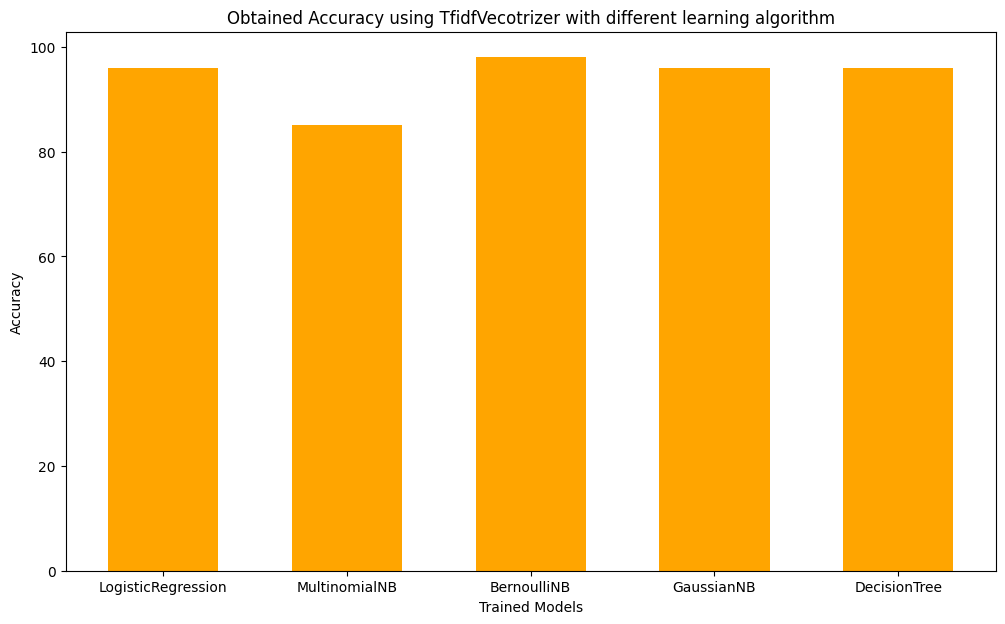
\includegraphics[scale=0.4]{Graphics/chart/tfidf_vect}
    \end{center}
    \caption{Accuracy using tfidf vectorizer for different Models}
    \label{fig:tfidf_vect_acc_chart}
\end{figure}

From the above graph we can see, except for one model, both tokenizers are equivalent and they are quite accurate in terms of detection
spam and non-spam email regardless of the model.
